While for many problem cases linear classifiers perform reasonable well, 
the restriction that purely linear decision boundaries for the classification can be modeled limit their scope of application.

This restriction was prominently demonstrated by \citet{MinskyPerceptrons}. They illustrated that for the different input combinations to the logical XOR operator, no linear decision boundary could be perceived for its outputs. A simple neural network may solve this problem. 
In the following section the boolean values True and False will be interchangeably used with their respective numeric representations 1 (True) and 0 (False).

The XOR operator is true if and only if one of two logical values on which this operator is used is true.

\begin{figure}[H]
  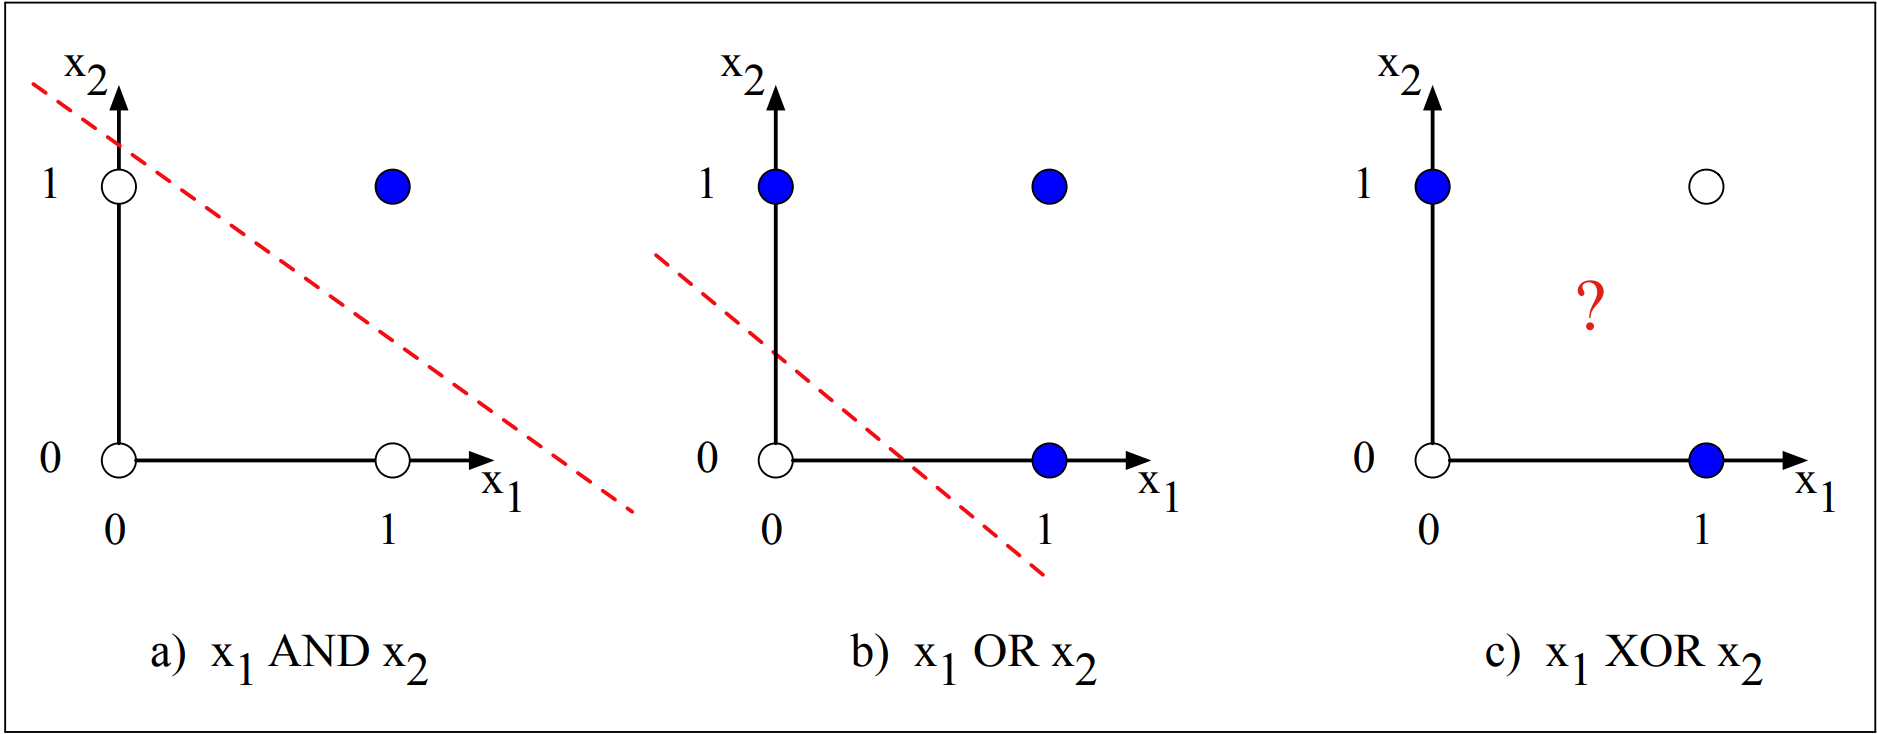
\includegraphics[width=\linewidth]{Pictures/Jurafsky_21_XOR_1.png}
  \caption{Adapted from \citet{jurafsky2021}: Visualisation of the logical functions a) AND, b) OR and c) XOR in a two dimensional space. If the points are blue the logical operator is True for this combination of truth values.}
  \label{fig:XOR1}
\end{figure}

In figure \ref{fig:XOR1}  three basic logical operators are shown in two-dimensional space where each axis represents the value of the boolean variables called $x_1, x_2$ respectively.
For the logical AND and OR one can easily assess that a linear decision boundary is conceivable. 
For the logical XOR on the other hand no decision boundary to separate the resulting boolean values can be reached in such a way.

Here the concept of layering multiple layers of processing units and applying non-linear functions on them can solve this. 
By adding a hidden layer the input values change eventually into a representation that is more favorable for basing a decision on.

\begin{figure}
  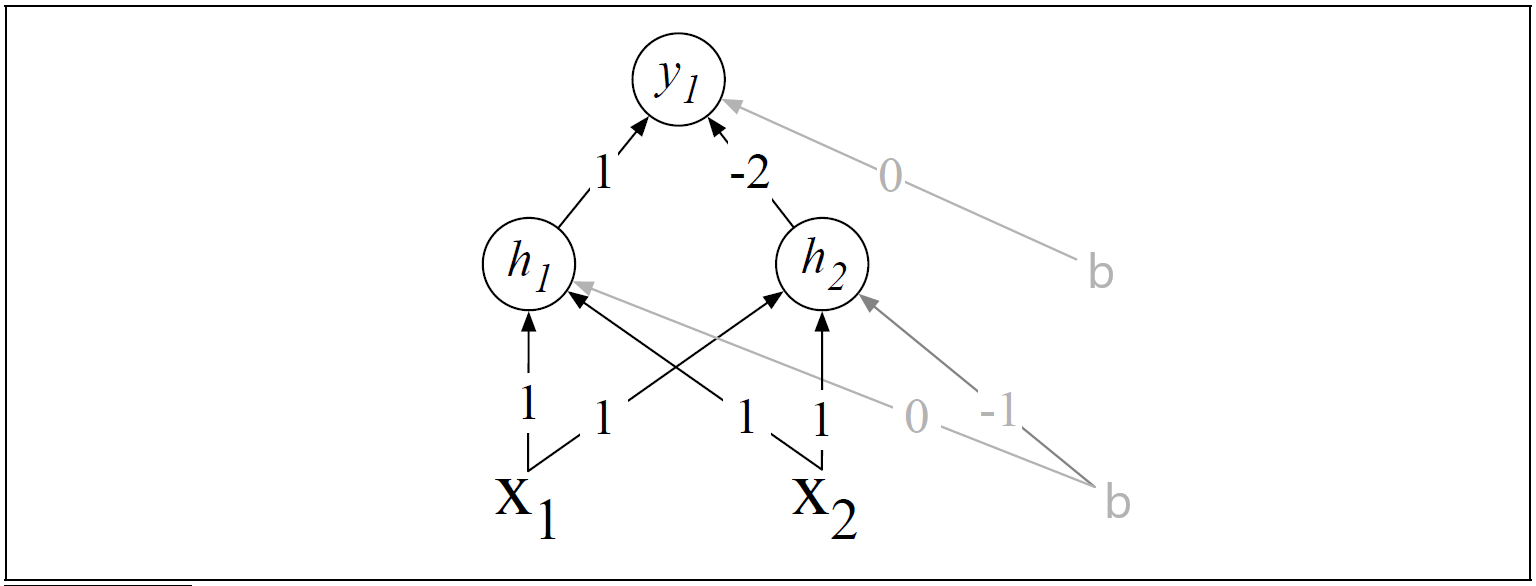
\includegraphics[width=\linewidth]{Pictures/Jurafsky_21_XOR_2.png}
  \caption{Adapted and modified from \citet{jurafsky2021}: Two-layer neural network to model the XOR operator}
  \label{fig:XOR2}
\end{figure}


Figure \ref{fig:XOR2} shows the processing units by circles with h inside for the hidden units and y for the output unit.
Weights are depicted by numbers on the black arrows and the value of the bias b for a unit by the number on a grey arrow.
Each unit multiplies the incoming values with the weights, sums them up, adds the bias and then returns the value if it is greater than 0, else 0 is given as its output. 
This filtering of outputs on whether the value is at least 0 is known as using the Rectified Linear Unit ($ReLU$) activation function which will be explored in more detail in \ref{nn_act}.

To give one example, in the case that both input variables $x_1,x_2$ are true, the input for this network is [1,1]. 
The computation that happens in $h_1$ is summing up $x_1$ times the weight from $x_1$ to $h_1$ (1*1), $x_2$ times the weight from $x_2$ to $h_1$ (1*1) and 
the bias that goes to $h_1$ (0) and afterwards returning 2 since this value is bigger than 0. 
In the second hidden node the computation happens similarly and its return value is 1. 
Therefore the input for the last layer which consists of only one unit $y_1$ which is called the output layer is [2,1]. 
Once the computation is finished for the last layer the return value is 0 which is the correct value in this case for the XOR operator. 

\begin{figure}
  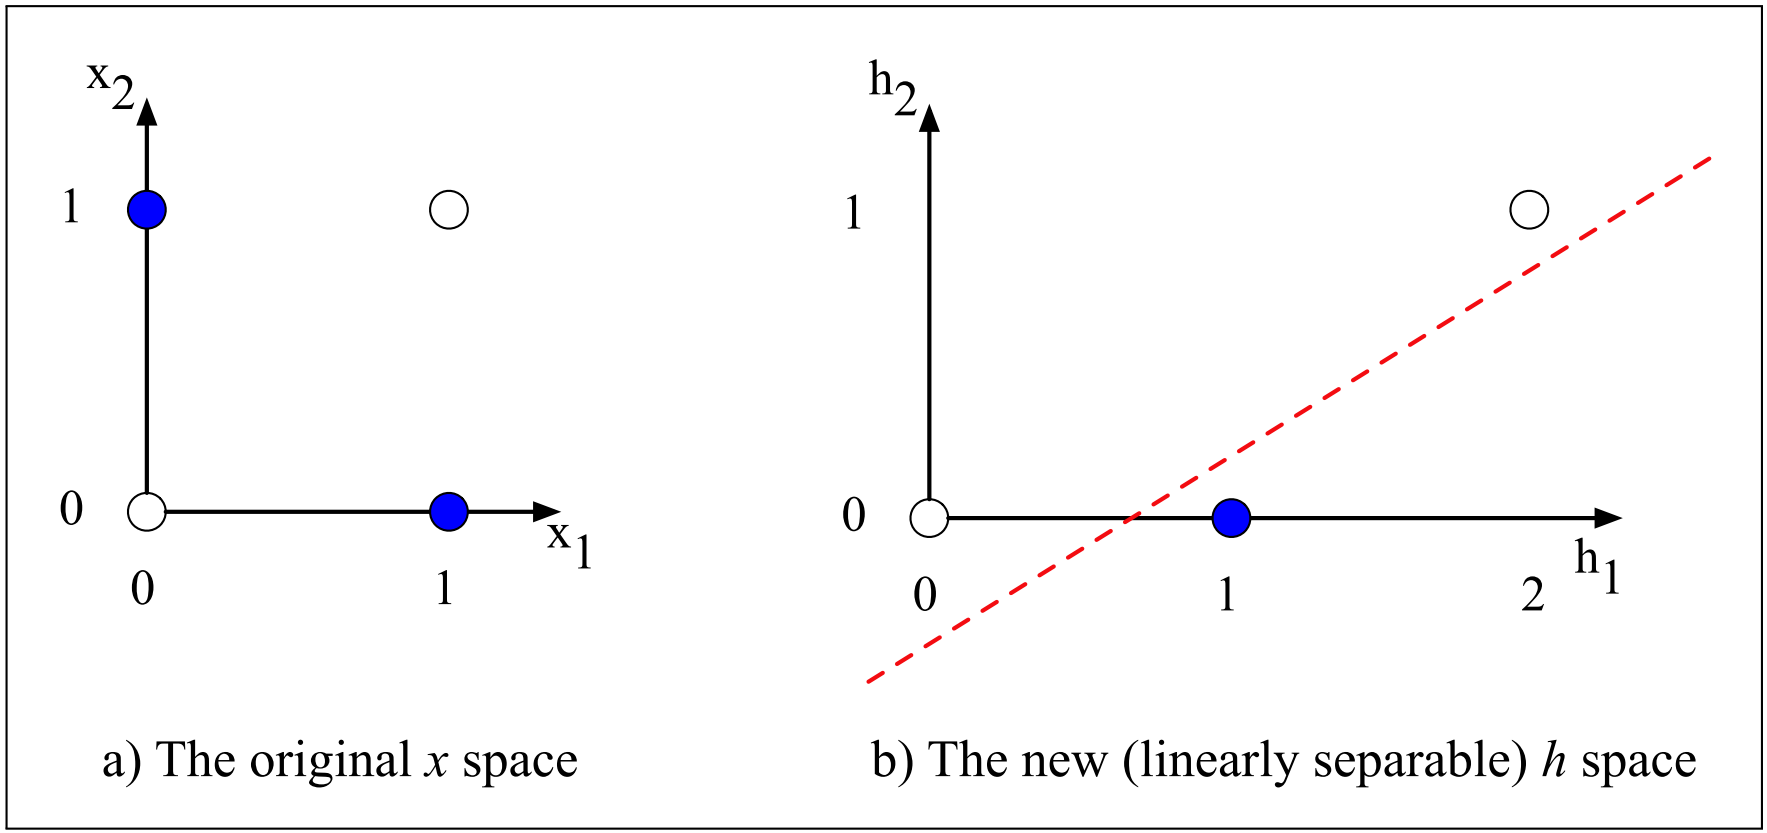
\includegraphics[width=\linewidth]{Pictures/Jurafsky_21_XOR_3.png}
  \caption{Adapted from \citet{jurafsky2021}: All cases for inputs to the XOR operator: a) are shown in their original configuration. b) have been transformed by passing the hidden layer (h) shown in Figure \ref{fig:XOR2}}
  \label{fig:XOR3}
\end{figure}

This can be done for all input combinations and it will return the appropriate value the XOR operator should return. 

After passing the hidden layer the input has been transformed into a different kind of representation of the data it held. 
If one computes the values of the hidden layer for all input combinations, the new resulting representation is linearly separable. 
Cases for which the XOR operator should return True have collapsed into the representation of [0,1] where the first value represents the first hidden unit's output and the second the other one. 
Figure \ref{fig:XOR3} shows the representation of data after the hidden layer for all cases. 
In b) we can now conceive a linear decision boundary which was not possible beforehand.

